\chapter{Introduction: Smartphone Market and the Need for Cross-Platform Support}
\label{chapter:introduction}

\section{Smartphone Landscape}
\label{section:smartphone-landscape}

\begin{table}
  \begin{tabular}{ l | l }
    \textbf{Mobile OS Type} & \textbf{Skill Set Required} \\
    \hline
    Apple iOS & C, Objective C \\
    Google Android & Java (Harmony flavored, Dalvik VM) \\
    RIM BlackBerry & Java (J2ME flavored) \\
    Symbian & C, C++, Python, HTML/CSS/JS \\
    Windows Mobile & .NET \\
    Windows 7 Phone & .NET \\
    HP Palm webOS & HTML/CSS/JS \\
    MeeGo & C, C++, HTML/CSS/JS \\
    Samsung bada & C++
  \end{tabular}
  \label{table:native-skills}
  \caption{Required skill sets for different mobile platforms. \cite{charland2011mobile}}
\end{table}

\section{HTML5}
\label{section:html5}

\subsection{History}
\subsection{Markup}
\subsection{CSS3}
\subsection{JavaScript APIs}
\subsection{Related APIs}

\section{Modern Mobile Web Application Architecture}
\label{section:modern-mobile-web}

\begin{figure}[ht]
  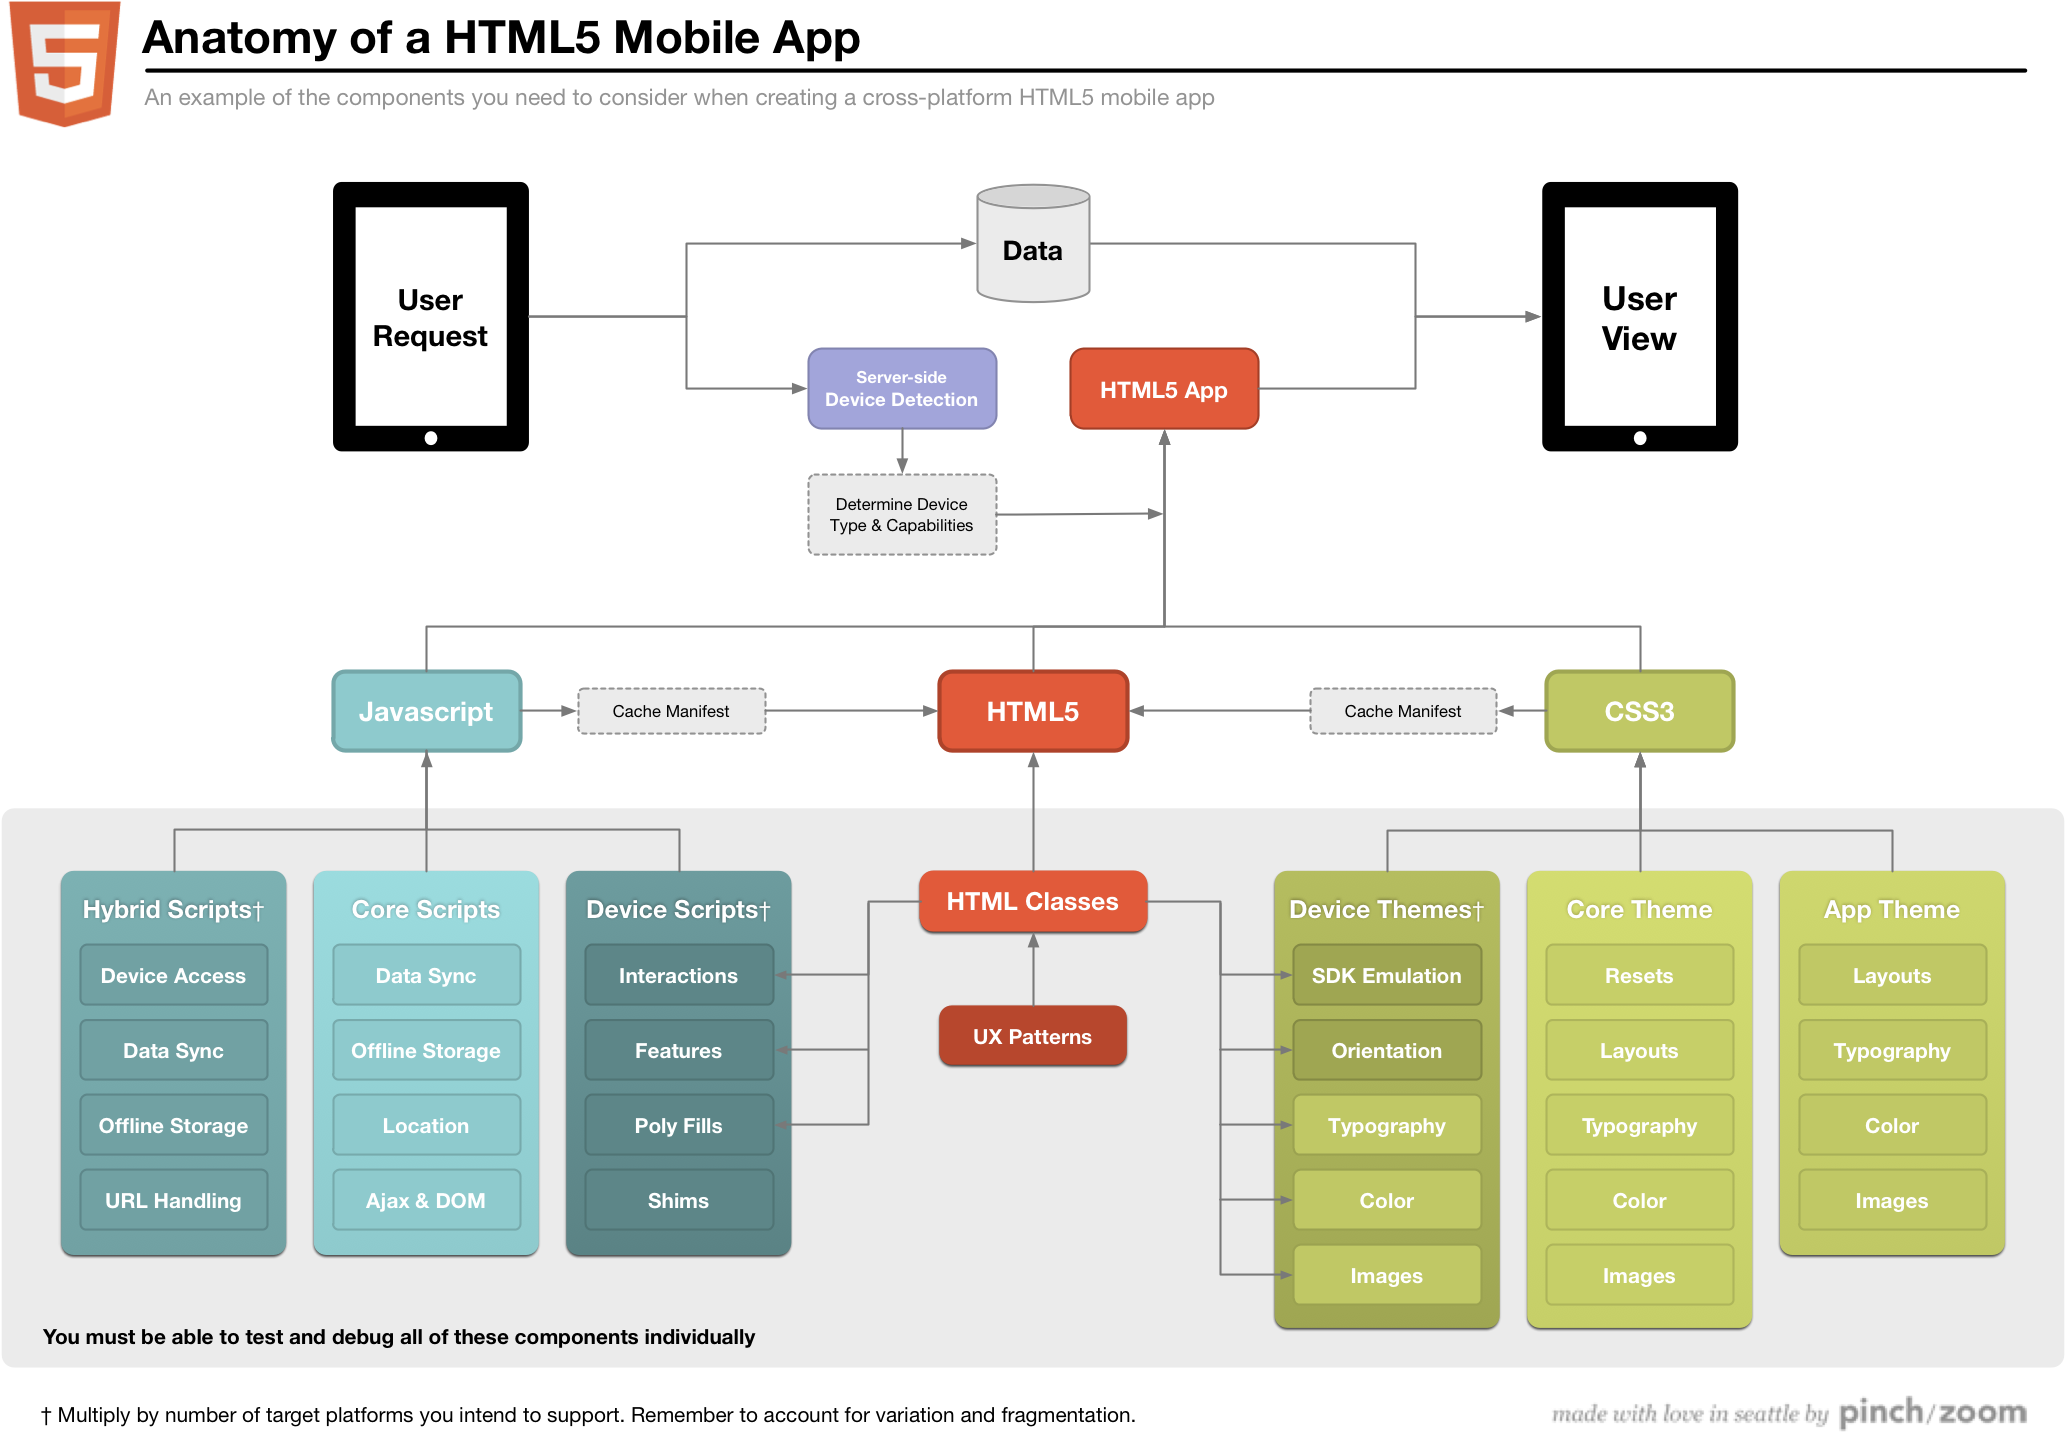
\includegraphics[width=\textwidth]{images/anatomy-of-a-html5-mobile-app.png}
  \caption{HTML5 Mobile Application Anatomy \citationneeded}
  \label{figure:anatomy-of-a-html5-mobile-app.png}
\end{figure}

\subsection{Single-Page applications}
\subsubsection{JavaScript MVC Libraries}

\subsection{Responsive Design}
\subsection{Progressive Enhancement}

\subsection{UI Libraries}
\subsubsection{jQuery Mobile}
\subsubsection{jQTouch}
\subsubsection{Sencha Touch}

\subsection{Hybrid Applications}
\subsection{Wrapping Web Applications Application Stores}

\clearpage
\section{Performance Guidelines}
\label{section:performance-guidelines}

\fixme{Add intro to sources and reasoning why frontend performance
  matters. \cite{souders2007high, souders2009even}}

\begin{itemize}
\item \textbf{Make Fewer HTTP Requests}



\item \textbf{Use a Content Delivery Network}



\item \textbf{Add an Expires Header}



\item \textbf{Gzip Components}



\item \textbf{Put Stylesheets at the Top}



\item \textbf{Put Scripts at the Bottom}



\item \textbf{Avoid CSS Expressions}



\item \textbf{Make Javascript and CSS External}



\item \textbf{Reduce DNS Lookups}



\item \textbf{Minify JavaScript}



\item \textbf{Avoid Redirects}



\item \textbf{Remove Duplicate Scripts}



\item \textbf{Configure ETags}



\item \textbf{Make Ajax Cacheable}



\item \textbf{Splitting the Initial Payload}



\item \textbf{Loading Scripts Without Blocking}



\item \textbf{Coupling Asynchronous Scripts}



\item \textbf{Positioning Inline Scripts}



\item \textbf{Writing Efficient JavaScript}



\item \textbf{Scaling with Comet}



\item \textbf{Going Beyond Gzipping}



\item \textbf{Optimizing Images}



\item \textbf{Sharding Dominant Domains}



\item \textbf{Flushing the Document Early}



\item \textbf{Using Iframes Sparingly}



\item \textbf{Simplifying CSS Selectors}



\end{itemize}
